\documentclass[tikz,border=10pt]{standalone}
\usepackage{amsmath,amssymb}
\usepackage{tikz}
\usetikzlibrary{shapes.geometric,arrows.meta,positioning,fit,backgrounds,calc,shadows}

\begin{document}
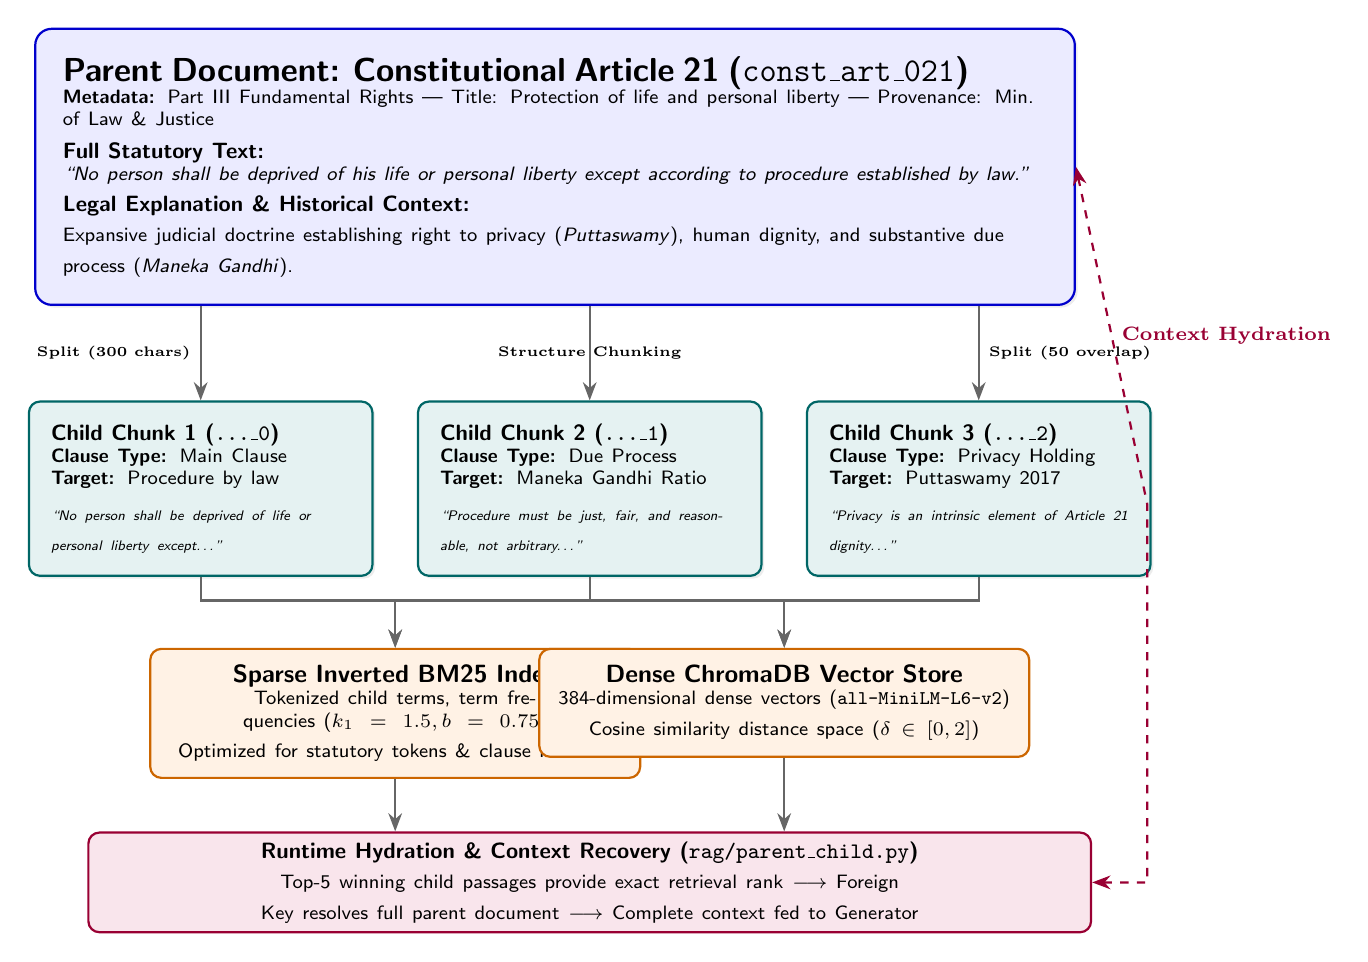
\begin{tikzpicture}[
    font=\sffamily\small,
    >=Stealth,
    node distance=0.8cm and 1.0cm,
    parentbox/.style={rectangle, draw=blue!80!black, fill=blue!8, rounded corners=6pt, thick, align=left, inner sep=10pt, drop shadow={opacity=0.15, shadow xshift=1pt, shadow yshift=-1pt}},
    childbox/.style={rectangle, draw=teal!80!black, fill=teal!10, rounded corners=4pt, thick, align=left, inner sep=8pt, drop shadow={opacity=0.15, shadow xshift=1pt, shadow yshift=-1pt}},
    indexbox/.style={rectangle, draw=orange!80!black, fill=orange!10, rounded corners=4pt, thick, align=center, inner sep=6pt},
    header/.style={font=\sffamily\bfseries\footnotesize, text=#1!80!black},
    flow/.style={->, thick, draw=gray!80!black},
    link/.style={<->, thick, dashed, draw=purple!80!black}
]

% Parent Document
\node[parentbox, text width=12.5cm] (parent) {
    \textbf{\large Parent Document: Constitutional Article 21 (\texttt{const\_art\_021})}\\
    \scriptsize \textbf{Metadata:} Part III Fundamental Rights | Title: Protection of life and personal liberty | Provenance: Min. of Law \& Justice\\
    \vspace{4pt}
    \textbf{\footnotesize Full Statutory Text:}\\
    \scriptsize \textit{``No person shall be deprived of his life or personal liberty except according to procedure established by law.''}\\
    \vspace{3pt}
    \textbf{\footnotesize Legal Explanation \& Historical Context:}\\
    \scriptsize Expansive judicial doctrine establishing right to privacy (\textit{Puttaswamy}), human dignity, and substantive due process (\textit{Maneka Gandhi}).
};

% Child Chunks
\node[childbox, text width=3.8cm, below=1.2cm of parent.south, xshift=-4.5cm] (c1) {
    \textbf{\footnotesize Child Chunk 1 (\texttt{\dots\_0})}\\
    \scriptsize \textbf{Clause Type:} Main Clause\\
    \scriptsize \textbf{Target:} Procedure by law\\
    \vspace{2pt}
    \tiny \textit{``No person shall be deprived of life or personal liberty except\dots''}
};

\node[childbox, text width=3.8cm, right=0.55cm of c1] (c2) {
    \textbf{\footnotesize Child Chunk 2 (\texttt{\dots\_1})}\\
    \scriptsize \textbf{Clause Type:} Due Process\\
    \scriptsize \textbf{Target:} Maneka Gandhi Ratio\\
    \vspace{2pt}
    \tiny \textit{``Procedure must be just, fair, and reasonable, not arbitrary\dots''}
};

\node[childbox, text width=3.8cm, right=0.55cm of c2] (c3) {
    \textbf{\footnotesize Child Chunk 3 (\texttt{\dots\_2})}\\
    \scriptsize \textbf{Clause Type:} Privacy Holding\\
    \scriptsize \textbf{Target:} Puttaswamy 2017\\
    \vspace{2pt}
    \tiny \textit{``Privacy is an intrinsic element of Article 21 dignity\dots''}
};

% Dual Indexing
\node[indexbox, text width=5.8cm, below=0.9cm of $(c1.south)!0.5!(c2.south)$] (bm25_idx) {
    \textbf{Sparse Inverted BM25 Index}\\
    \scriptsize Tokenized child terms, term frequencies ($k_1=1.5, b=0.75$)\\
    \scriptsize Optimized for statutory tokens \& clause numbers
};

\node[indexbox, text width=5.8cm, below=0.9cm of $(c2.south)!0.5!(c3.south)$] (chroma_idx) {
    \textbf{Dense ChromaDB Vector Store}\\
    \scriptsize 384-dimensional dense vectors (\texttt{all-MiniLM-L6-v2})\\
    \scriptsize Cosine similarity distance space ($\delta \in [0, 2]$)
};

% Recovery / Hydration banner
\node[rectangle, draw=purple!80!black, fill=purple!10, rounded corners=4pt, thick, text width=12.5cm, align=center, below=0.8cm of $(bm25_idx.south)!0.5!(chroma_idx.south)$] (recovery) {
    \textbf{\footnotesize Runtime Hydration \& Context Recovery (\texttt{rag/parent\_child.py})}\\
    \scriptsize Top-5 winning child passages provide exact retrieval rank $\longrightarrow$ Foreign Key resolves full parent document $\longrightarrow$ Complete context fed to Generator
};

% Arrows
\draw[flow] (parent.south -| c1.north) -- (c1.north) node[midway, left, font=\tiny\bfseries] {Split (300 chars)};
\draw[flow] (parent.south -| c2.north) -- (c2.north) node[midway, font=\tiny\bfseries] {Structure Chunking};
\draw[flow] (parent.south -| c3.north) -- (c3.north) node[midway, right, font=\tiny\bfseries] {Split (50 overlap)};

\draw[flow] (c1.south) -- ++(0,-0.3) -| (bm25_idx.north);
\draw[flow] (c2.south) -- ++(0,-0.3) -| (bm25_idx.north);
\draw[flow] (c2.south) -- ++(0,-0.3) -| (chroma_idx.north);
\draw[flow] (c3.south) -- ++(0,-0.3) -| (chroma_idx.north);

\draw[flow] (bm25_idx) -- (bm25_idx |- recovery.north);
\draw[flow] (chroma_idx) -- (chroma_idx |- recovery.north);
\draw[link] (recovery.east) -- ++(0.7,0) -- ++(0,4.8) -- (parent.east) node[midway, right, font=\scriptsize\bfseries, text=purple!80!black] {Context Hydration};

\end{tikzpicture}
\end{document}
